\documentclass[12pt]{article}

\usepackage{report}

\usepackage[utf8]{inputenc} % allow utf-8 input
\usepackage[T1]{fontenc}    % use 8-bit T1 fonts
\usepackage[colorlinks=true, linkcolor=black, citecolor=blue, urlcolor=blue]{hyperref}       % hyperlinks
\usepackage{url}            % simple URL typesetting
\usepackage{booktabs}       % professional-quality tables
\usepackage{amsfonts}       % blackboard math symbols
\usepackage{nicefrac}       % compact symbols for 1/2, etc.
\usepackage{microtype}      % microtypography
\usepackage{lipsum}		% Can be removed after putting your text content
\usepackage{graphicx}
\usepackage{natbib}
\usepackage{doi}
\usepackage{listings}
\usepackage{xcolor}
\usepackage{float}
\setcitestyle{aysep={,}}



\title{Project Step 3}

\author{Brian Lee, Chloe Gentry, Vinny Rose\\
\AND\\
\AND
\AND
\AND
\AND
	CS.3339 Computer Architecture\\
\AND
	Texas State University\\
}

% Uncomment to remove the date
\date{December 3, 2024}

% Uncomment to override  the `A preprint' in the header
\renewcommand{\headeright}{Project Step 3 - Group Name}
\renewcommand{\undertitle}{Smarty Pants}
\renewcommand{\shorttitle}{}

\definecolor{codegreen}{rgb}{0,0.6,0}
\definecolor{codegray}{rgb}{0.5,0.5,0.5}
\definecolor{codepurple}{rgb}{0.58,0,0.82}
\definecolor{backcolour}{rgb}{0.95,0.95,0.92}

\lstdefinestyle{mystyle}{
    backgroundcolor=\color{backcolour},   
    commentstyle=\color{codegreen},
    keywordstyle=\color{magenta},
    numberstyle=\tiny\color{codegray},
    stringstyle=\color{codepurple},
    basicstyle=\ttfamily\footnotesize,
    breakatwhitespace=false,         
    breaklines=true,                 
    captionpos=b,                    
    keepspaces=true,                 
    numbers=left,                    
    numbersep=5pt,                  
    showspaces=false,                
    showstringspaces=false,
    showtabs=false,                  
    tabsize=2
}

\lstset{style=mystyle}


\begin{document}
\maketitle

\newpage
\tableofcontents
\thispagestyle{empty}


\newpage
\setcounter{page}{1}
\section{Introduction}
In this project, we explored a comprehensive Verilog-based implementation and testing process for logical, arithmetic, and shift operations. The conversation covered the design of modular Verilog components, including logic gates, arithmetic units, and shifters, as well as their integration into a testbench. Each module was designed to handle specific operations like addition, subtraction, and various shift types, ensuring clear functionality and reusability. The testbench applied rigorous testing using various input cases, including edge scenarios, and captured results in both display outputs and waveform files for simulation.

Next, we tested each circuit's functionality to ensure expected behavior, followed by generating simulation waveforms to visually confirm the ALU’s performance. Finally, we compiled our work and observations into a comprehensive report, which summarizes the methods, results, and key insights gained from the project.


\section{Logic circuit}
This Verilog code defines a Logic Unit with both single-bit and 4-bit modules for performing logical operations such as AND, NAND, OR, NOR, XOR, XNOR, and NOT. Each operation is implemented as a separate module for modularity and ease of testing.
\subsection{Logic Circuit code}
\lstinputlisting[language=Verilog]{logic_unit.v}

\subsection{Logic Waveforms}
\begin{figure}[H]
    \centering 
   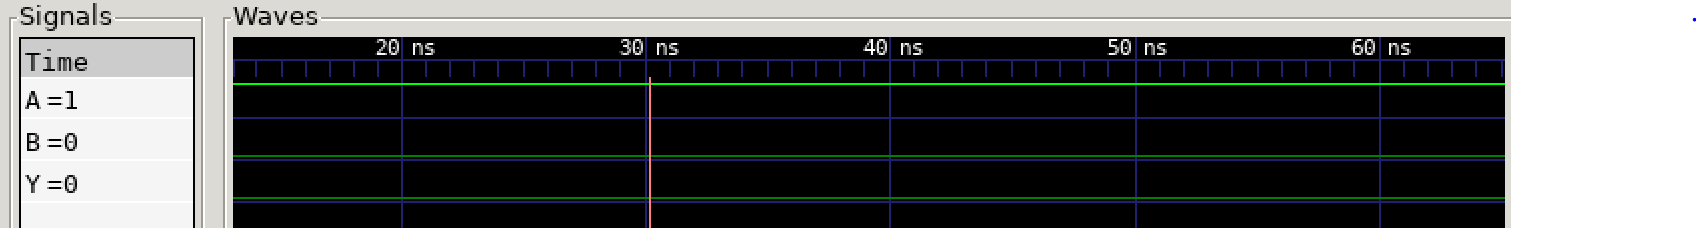
\includegraphics[width = 1.0\textwidth]{pictures/1bitNor.PNG}
    \caption{1-bit Nor wave form}
    \label{fig:enter-label}
    \end{figure}

\begin{figure}[H]
    \centering 
    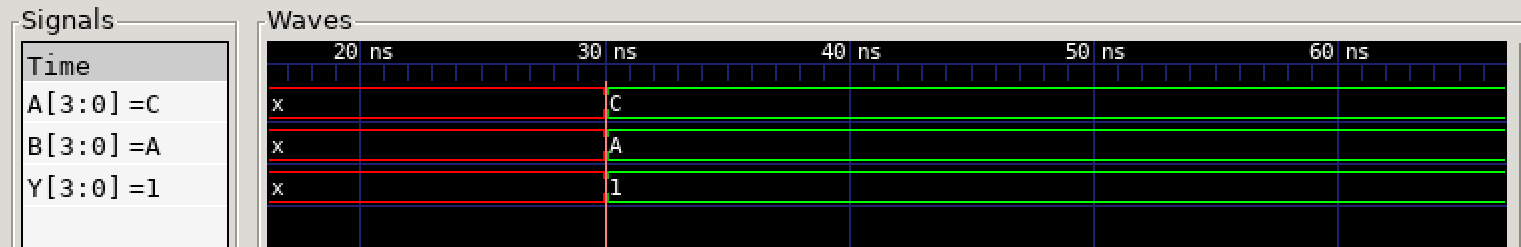
\includegraphics[width = 1.0\textwidth]{pictures/4bitNor.PNG}
    \caption{4-bit Nor wave form}
    \label{fig:enter-label}
    \end{figure}   

\begin{figure}[H]
    \centering 
    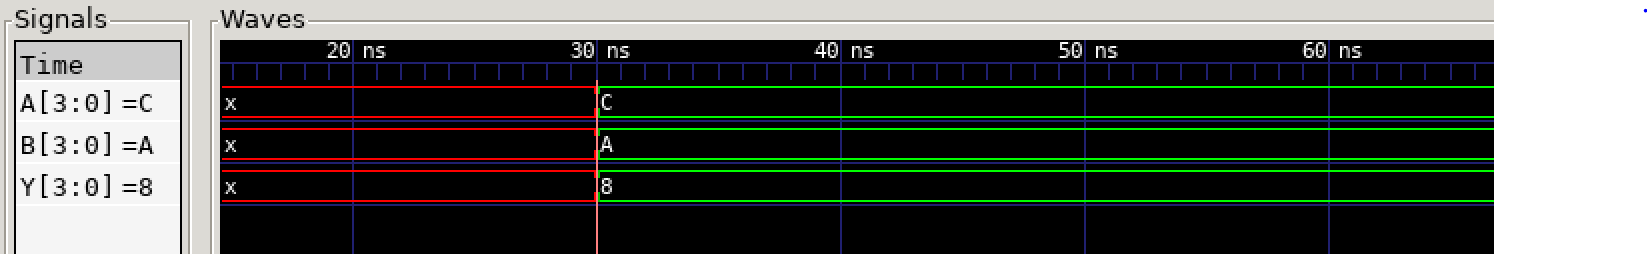
\includegraphics[width = 1.0\textwidth]{pictures/4bitAnd.PNG}
    \caption{4-bit And wave form}
    \label{fig:enter-label}
    \end{figure} 


\section{Alu circuit}
This Verilog code defines an Arithmetic Logic Unit (ALU) with modular functionality for addition, subtraction, multiplication, and division. Each operation is implemented as a separate module, and a 4-bit opcode determines the operation to execute. The ALU produces outputs such as the arithmetic result, carry-out for addition, product (high and low bits) for multiplication, quotient, remainder, and validity for division. The design promotes modularity and flexibility, making it easy to test and extend.
\subsection{ALU circuit code}
\lstinputlisting[language=Verilog]{alu.v}

\subsection{ALU Waveforms}
\begin{figure}[H]
    \centering 
   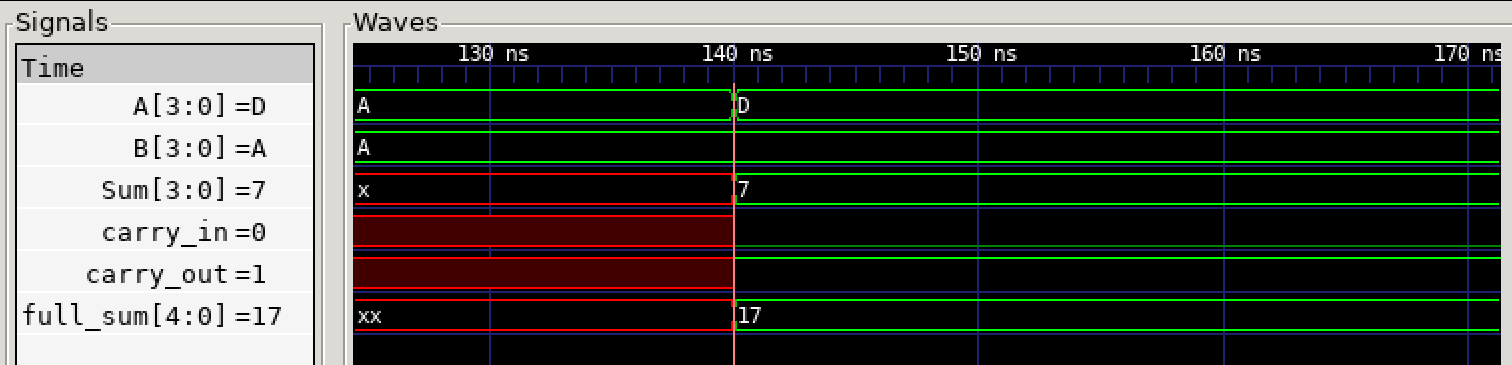
\includegraphics[width = 1.0\textwidth]{pictures/4bitAddition.PNG}
    \caption{4-bit Addition wave form}
    \label{fig:enter-label}
    \end{figure}

\begin{figure}[H]
    \centering 
    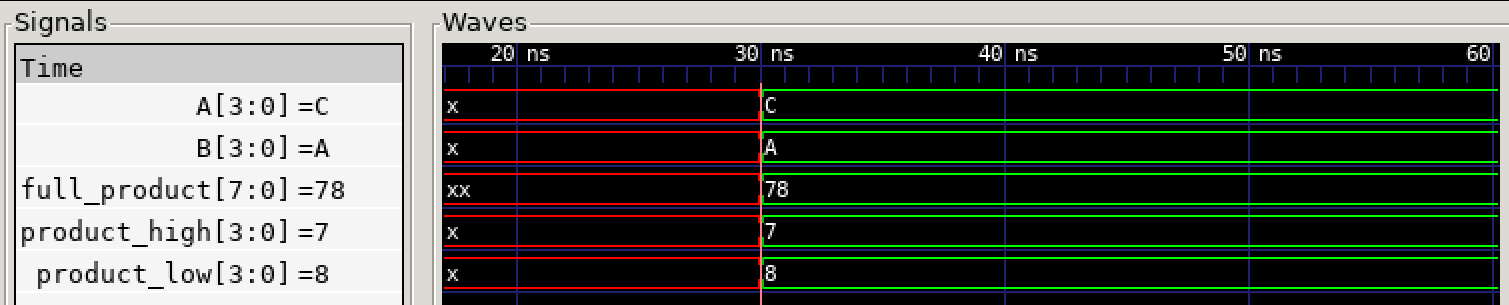
\includegraphics[width = 1.0\textwidth]{pictures/4bitMultiplication.PNG}
    \caption{4-bit Multiplication wave form}
    \label{fig:enter-label}
    \end{figure}   

\begin{figure}[H]
    \centering 
    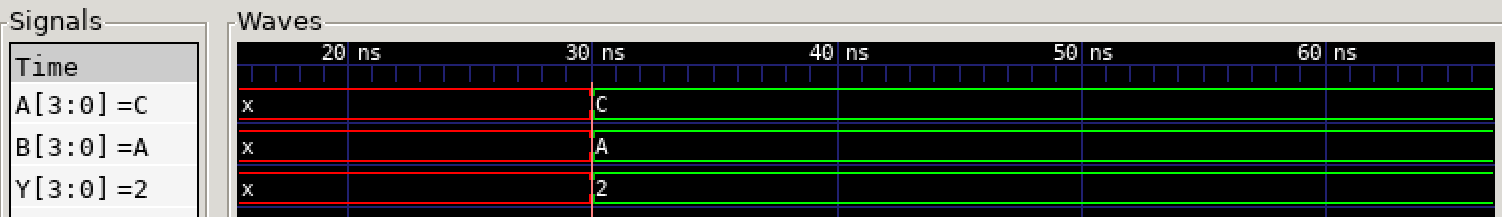
\includegraphics[width = 1.0\textwidth]{pictures/4bitSubtraction.PNG}
    \caption{4-bit Subtraction wave form}
    \label{fig:enter-label}
    \end{figure} 

\section{Shift circuit}
The provided Verilog code defines two modules for bit shifting operations. A 1 bit shift and a 2 by 4 bit shift
\subsection{Shifter circuit code}
\lstinputlisting[language=Verilog]{shifter.v}

\subsection{Shift Waveform}
\begin{figure}[H]
    \centering 
   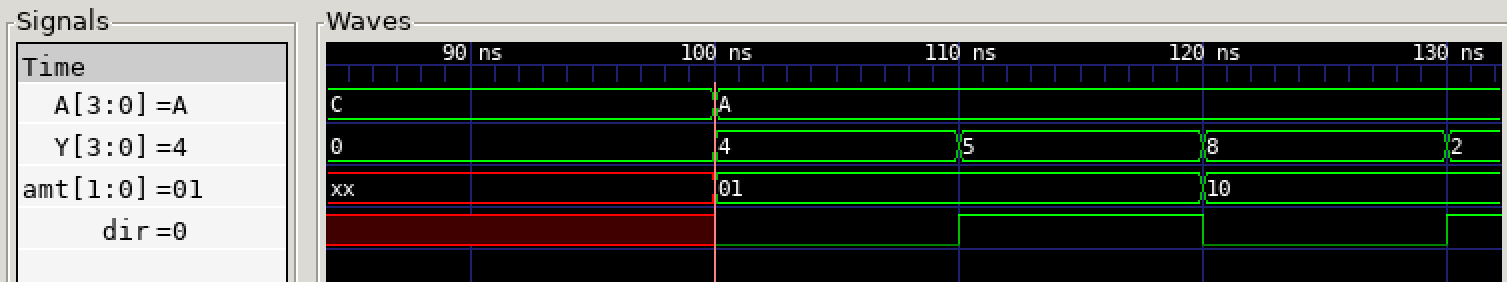
\includegraphics[width = 1.0\textwidth]{pictures/4bitShift.PNG}
    \caption{4-bit Shift wave form}
    \label{fig:enter-label}
    \end{figure}

\section{Testbench circuit}
This Verilog testbench evaluates logical, arithmetic, and shift operations across multiple modules. It tests single-bit and 4-bit logical operations, including AND, OR, NOT, XOR, and their variations, as well as addition, subtraction, multiplication, and division with detailed result validation. Shift operations are tested for both single-bit and multi-bit shifts in left and right directions.
\subsection{Testbench circuit code}
\lstinputlisting[language=Verilog]{testbench.v}

\section{Opcode Module}
\begin{figure}[H]
    \centering 
   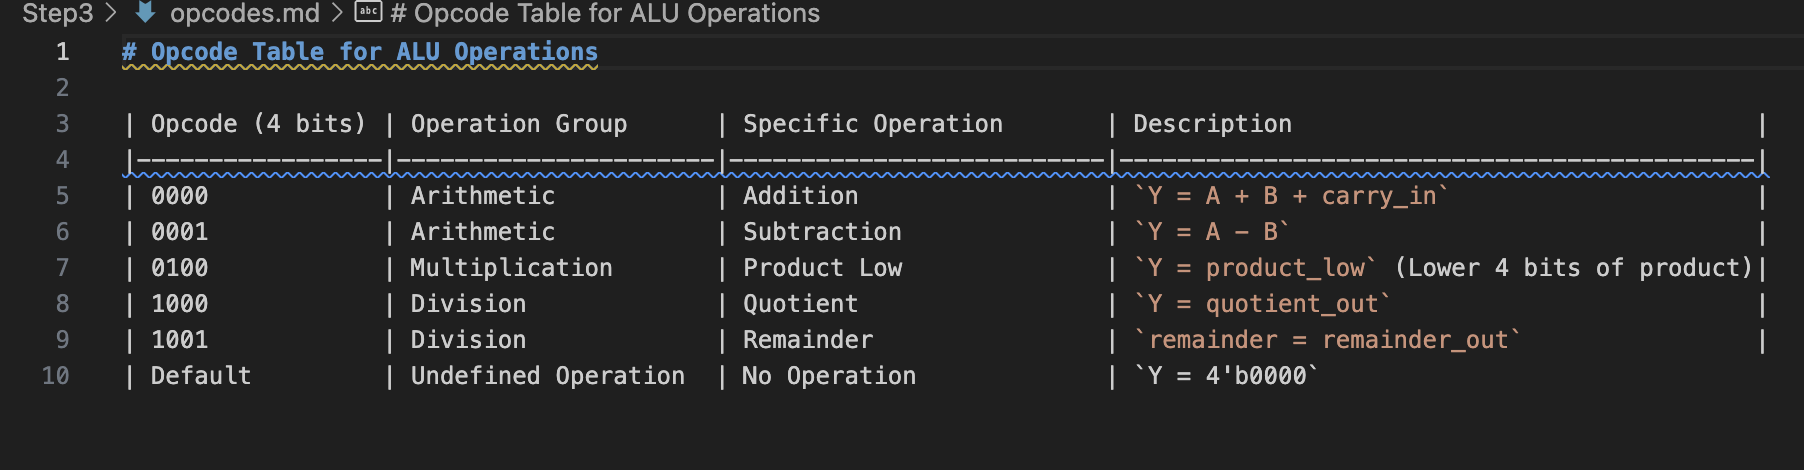
\includegraphics[width = 1.0\textwidth]{pictures/Opcode.png}
    \caption{Opcode Screenshot}
    \label{fig:enter-label}
    \end{figure}

\section{Conclusion}

This project introduced the design and testing of a Arithmetic Logic Unit (ALU), logic unit, and shifting unit. We coded essential logic functions like AND, OR, and NOT, along with shifting operations, which are crucial for handling binary data. We also developed basic arithmetic operations—addition, subtraction, multiplication, and division—which included handling carries and remainders to ensure accurate results.

Testing the circuits and generating waveforms confirmed that our ALU worked correctly across different inputs. This process highlighted the importance of both accuracy in coding and thorough testing. Overall, the project has been valuable for understanding digital circuits and the structure of an ALU, preparing us for more advanced digital logic design.
\end{document}



